\documentclass[twocolumn,onesided,9pt]{article}

\usepackage{./Task32FlyerLatexStyle/Task32Flyer}

%% -----------------------------------
%% Document information
%% -----------------------------------
\def\pubdate{17 September 2019}
\title{Increasing the impact of wind lidar through digitalisation}
\shorttitle{Increasing the impact of wind lidar through digitalisation}
\DOI{10.5281/zenodo.3447756}
\version{1.1}
\addbibresource{bibliography}

%% ===================================
%% Document starts
%% ===================================

\begin{document}

%% -----------------------------------
%% Title
%% -----------------------------------
\maketitle
\thispagestyle{cover}

%% -----------------------------------
%% Introductory text
%% -----------------------------------
{\Large\noindent%
What is digitalisation, how does it help wind lidar and wind energy, and how can we make it happen?
}
\vskip 6pt

Wind lidar can help to improve wind energy resource assessment campaigns, to increase plant performance, and to reduce operations \& maintenance costs \cite{Clifton_2018_a}. Digitalisation is modifying processes and disrupting businesses in many sectors, including wind energy \cite{TP-5000-68123}. This white paper provides an overview of how digitalisation could help the wind energy industry benefit from wind lidar, and what needs to be done to make this vision a reality.

\section*{What does digitalisation mean for wind lidar?}
Digitalisation has many different meanings. It means that hardware is designed for two-way communications and can be controlled remotely. It also means that knowledge that was on paper or in users' heads is captured in software. This in turn allows experience to be shared across the community. It then allows digital workflows that add value for users. Furthermore, it means that the data from such devices are created with the FAIR principles in mind, i.e. that the data should be findable, accessible, interoperable, and reusable. Digitalised devices can become part of collaborative workflows, allowing more value to be extracted from their data.

\section*{How does wind energy benefit from the digitalisation of wind lidar?}
Digitalisation of wind lidar allows the growth of an ecosystem of products and services that use the much increased knowledge about wind plant conditions. Digitalisation is thus most powerful when it is backed by community standards that allow communication and collaboration. For example:
\begin{itemize}
    \item Lidar-specific communication protocols allow users to manage lidars for wind turbine or wind park control, or for specific measurements (Figure \ref{fig:lotsOfLidar}). 
    \item Data created using standard data formats can be stored, found, and retrieved easily. Data stored in these formats can then be exchanged between different users without losing information. And, analysis codes can read these formats directly, which removes the need for device-specific import filters.
    \item Stable data analysis process allow users to create physics-based uncertainty estimates and calibrate them using field data. These may be lower than experience-based estimates in some cases.
    \item Experience can be captured in software tools, such as for planning measurement campaigns \cite{wes-2019-13} or data analysis. This makes it easier to build processes and improve them over time.
    \item Standardized communication and data formats reduce the barriers to deploying wind lidar, which results in a virtuous cycle of reduced user costs and further increased wind lidar deployment.
    \item Lidar can become modular, changing configuration as needed. This was the core of the OpenLidar concept developed by members of Task 32 in 2015 (Fig. \ref{fig:OpenLidar}). For example, the same core Doppler wind lidar unit could be used as part of a scanning lidar \cite{Wuerth_2017_3416356}, flown on a drone \cite{amt-2019-102}, or included in a floating lidar system  \cite{Bischoff_2017_a}. Modular design helps when developing new products and applications, while modular construction simplifies maintenance.
\end{itemize}

Digitalisation thus offers the potential to deploy improved wind lidar for more accurate resource assessment campaigns, to increase plant performance and energy capture, and to reduce operations \& maintenance costs. It also offers less experienced lidar users ways to leverage others' expertise.

\begin{figure}[htb]
    \centering
    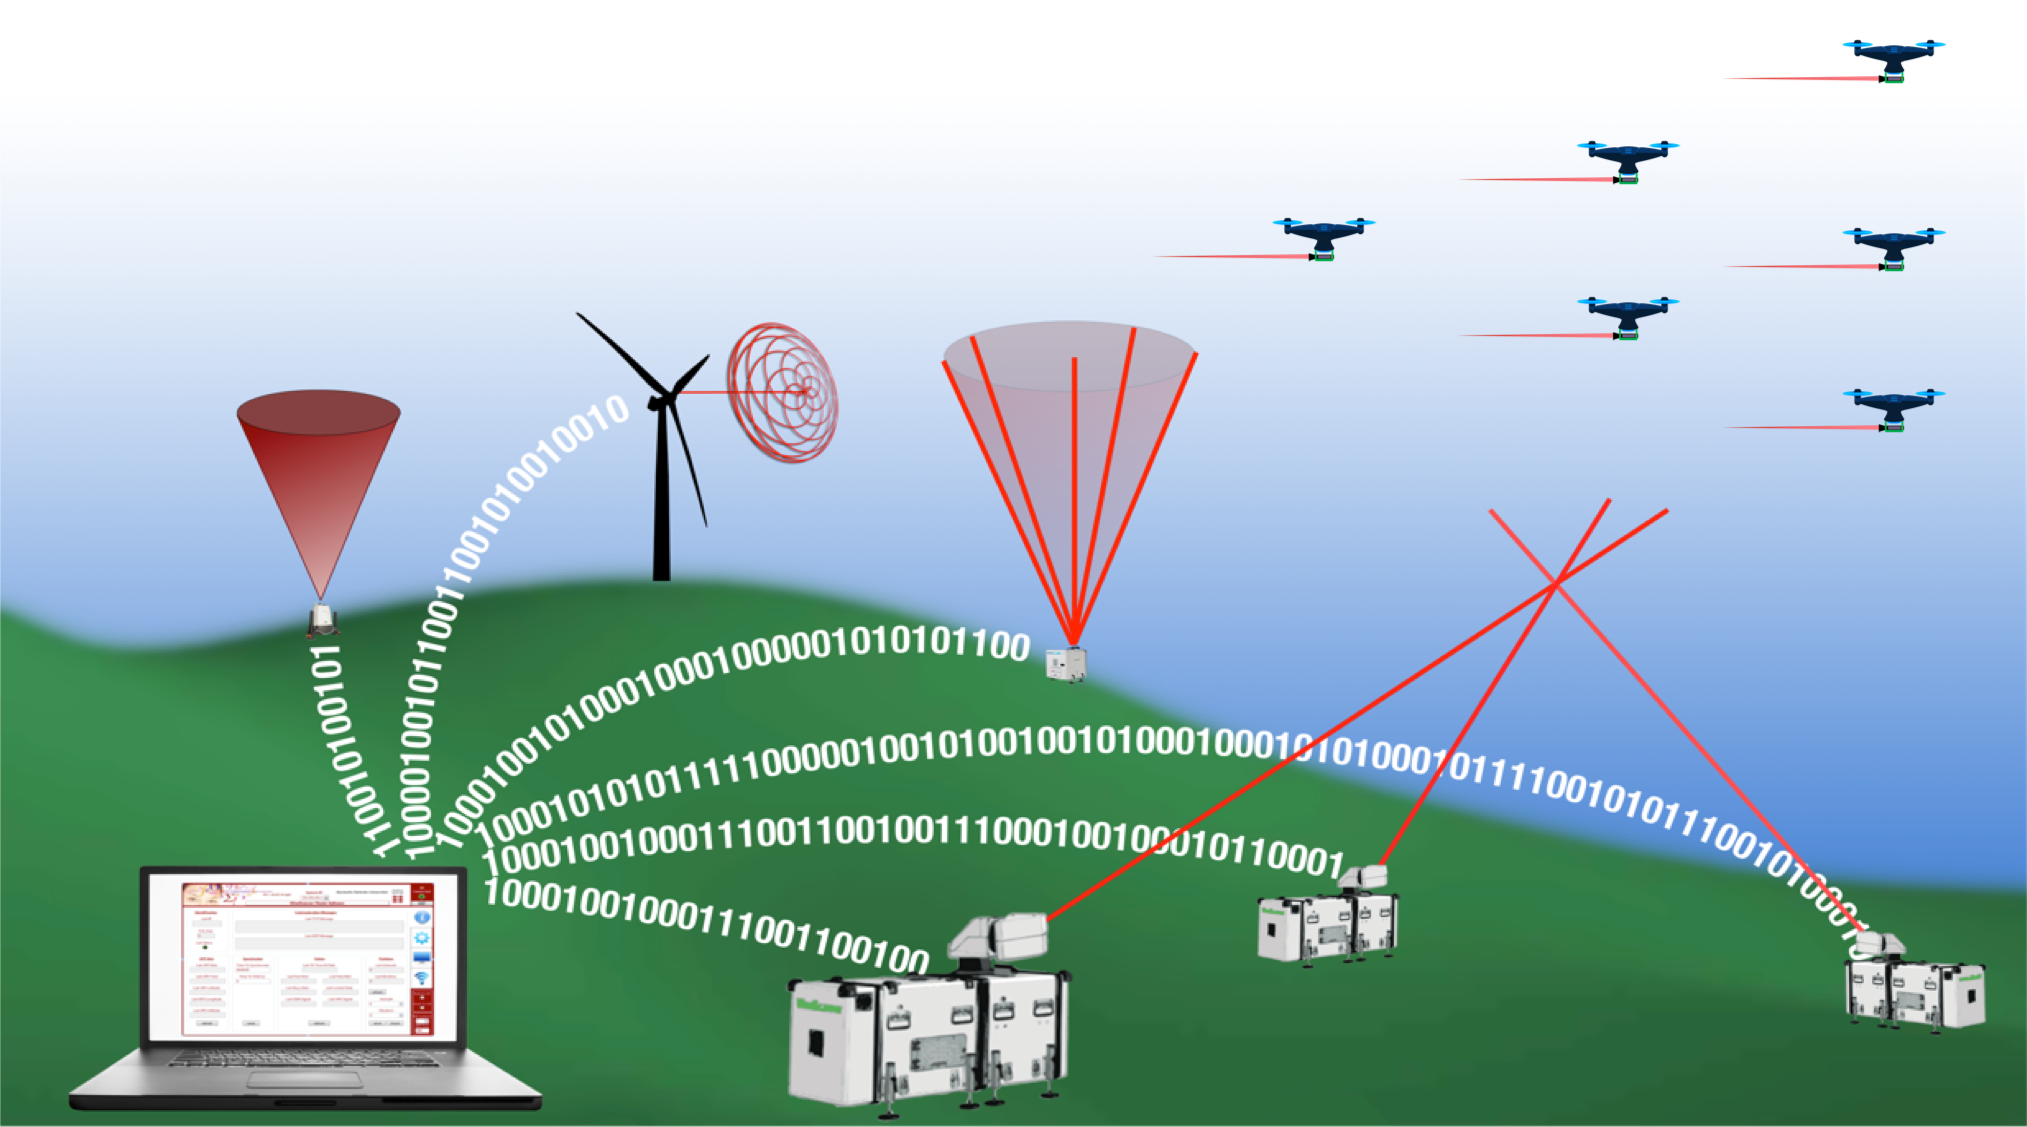
\includegraphics[width=0.95\linewidth]{graphics/digit_lid.png} 
    \caption{Many different types of wind lidar can be used together to give unprecedented insight into the wind conditions in and around a wind plant.}
    \label{fig:lotsOfLidar}
\end{figure}
    
\begin{figure}[hbt]
    \centering
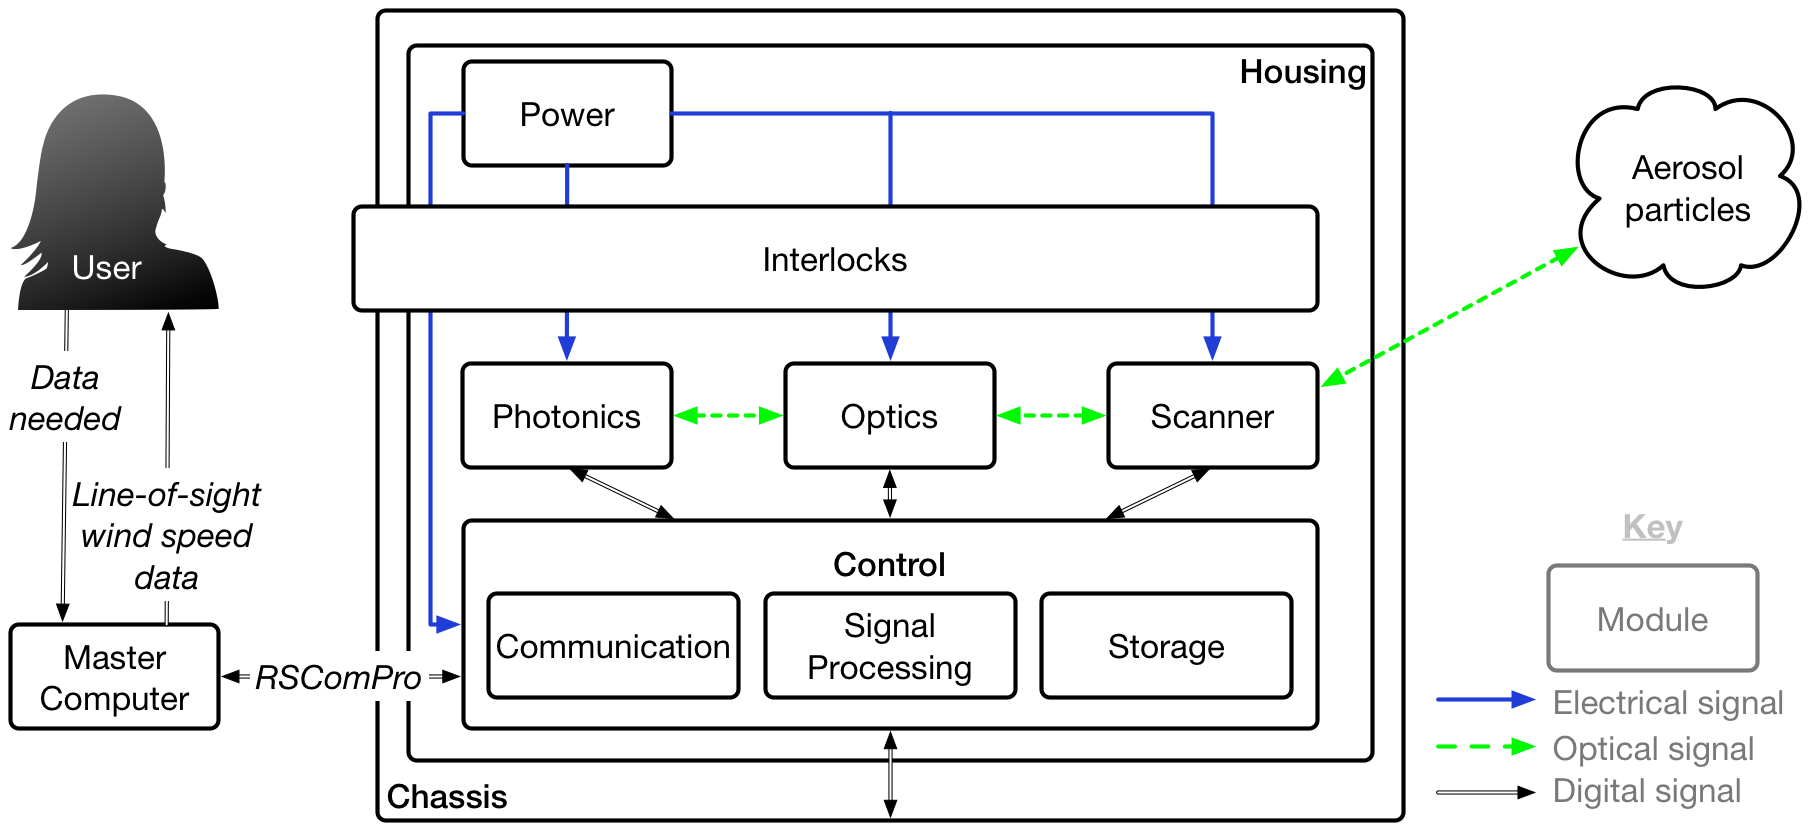
\includegraphics[width=0.95\linewidth]{graphics/OpenLidarModules.png} 
\caption{The OpenLidar modular wind lidar concept uses digitalisation to enable innovation in wind lidar \protect{\cite{Wuerth_2017_3416356}}}
\label{fig:OpenLidar}
\end{figure}

\section*{How can we prepare for digitalisation?}
Digitalisation offers many benefits to individual users but also becomes more powerful as more of the community adopts it. Many actors in the wind lidar community have already embraced the benefits offered by the digitalisation of wind lidar. But, there are still steps that need to be taken by different groups.

% vendors
Almost all \textbf{lidar vendors} allow communications with their lidar through a remote desktop or a proprietary graphical interface. Application Programming Interfaces (APIs) or communications using defined protocols such as RSComPro \cite{Vasiljevic_2013_RSComPro} are less common but their availability would enable multiple lidars to be used together. Also, most vendors use proprietary data formats. This requires import filters for each device and causes uncertainty about the data. This could be avoided by using the e-WindLidar data formats \cite{Vasiljevic_2018_2478051}, which define XML data formats for specific data `levels' or points in data processing.

% system integrators
Many lidar devices are integrated into other systems, for example into wind turbines for wind turbine control, or as part of floating lidar systems. \textbf{System integrators} and \textbf{wind turbine OEMs} could encourage vendors to use standard communication protocols and data formats to simplify integration.

% data users
\textbf{Data users} should adopt the e-WindLidar data formats. This will encourage vendors to provide data in those formats, and encourage the development of third-party tools to analyse the data.

% researchers
\textbf{Researchers} use many different wind lidar. Researchers could store data using an open format and develop reusable, modular analysis codes that leverage those formats. Researchers should be supported to share the results of publicly-funded research in public repositories. This would help innovation and technology transfer.

% community groups
\textbf{Community groups and standards bodies} such as IEA Wind Task 32, the Consortium for the Advancement of Remote Sensing (CFARS), MEASNET, and others should encourage stakeholders to adopt common and interoperable standards for communication and data. This will provide the market ``pull'' for such products and encourage the creation of an ecosystem.

% service providers
\textbf{Service providers} need to provide tools that enable and leverage digitalisation. For example, secure environments where data from multiple sources and owners can be brought together, analysed, and acted upon will be crucial. Collaborative data platforms need to be made easier to use to accelerate their adoption.

% avoid new heading at the end of the column
\newpage

\section*{Conclusions}
Digital wind lidar offer many advantages for wind energy applications. Many of the tools that are needed already exist. An ecosystem of products and services will be enabled by new approaches to hardware and software. Task 32 and other groups will be essential in bringing stakeholders together to establish consensus and help speed up the process. 

%% -----------------------------------
%% References
%% -----------------------------------
%\section*{References}
% bibliography
\label{sec:References}
\addcontentsline{toc}{section}{References}
\defbibnote{openaccess}{The following documents are all open access.}
{\small
\printbibliography%[prenote=openaccess]
}

%% -----------------------------------
%% Outlined block of smaller text
%% -----------------------------------
\begin{tcolorbox}[width=1.0\columnwidth,
                  boxsep=0pt,
                  left=3pt,
                  right=3pt,
                  top=3pt,
                  arc=0pt,
                  boxrule=0.5pt,
                  toprule=0.5pt,
                  colback=white,
                  coltext=TextGrey,
                  code={\linespread{1.0}}
                  ]
{\footnotesize%
This white paper was self published by IEA Wind Task 32.}

%% -----------------------------------
%% IEA WIND AND TASK 32
%% -----------------------------------
\begin{tabular}{m{0.3\columnwidth}m{0.6\columnwidth}}
    % IEA Wind * DO NOT EDIT THIS TEXT *
    
\includegraphics[height=2cm]{graphics/IEAWind_logo.jpg} &
    {\footnotesize%
    The International Energy Agency is an autonomous organisation which works to ensure reliable, affordable and clean energy for its 30 member countries and beyond. The IEA Wind Technology Collaboration Programme supports the work of 38 independent, international groups of experts that enable governments and industries from around the world to lead programmes and projects on a wide range of energy technologies and related issues.}  %
    \\
    % Task 32 * DO NOT EDIT THIS TEXT *
    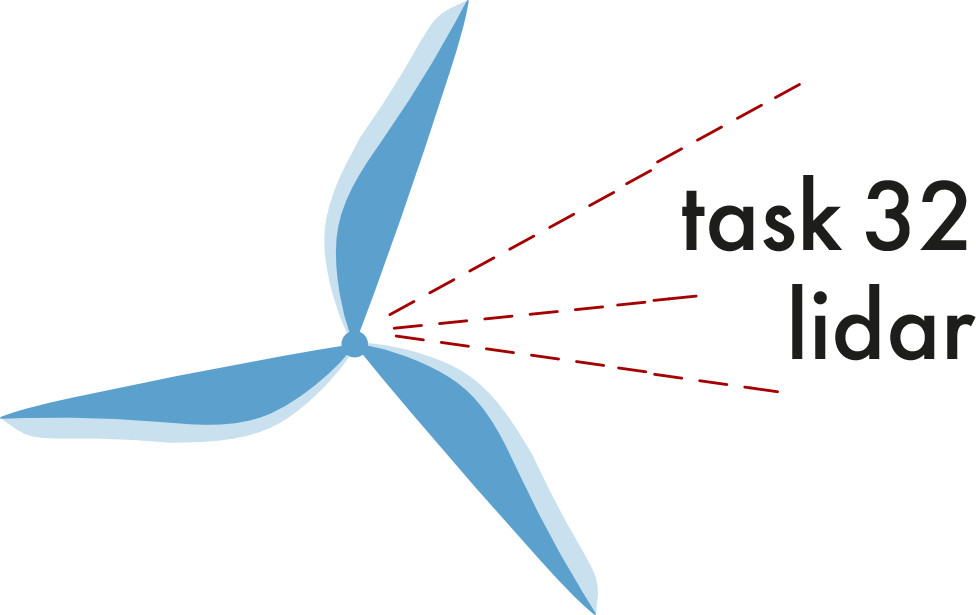
\includegraphics[height=1.5cm]{graphics/Task32_logo.jpg} &
    {\footnotesize%
    \href{www.ieawindtask32.org}{IEA Wind Task 32} is a community that aims to identify and mitigate the barriers to the deployment of wind lidar for wind energy applications.}
\end{tabular}%

%% -----------------------------------
%% For more information
%% -----------------------------------
% N.B. do not add line breaks between the next items
{\footnotesize%
\textbf{For more information:} %
Many of the tools mentioned here are archived in the \href{https://github.com/e-WindLidar}{GitHub e-WindLidar repository}.
%% -----------------------------------
%% Authors
%% -----------------------------------
\textbf{Author team:} %
Andrew Clifton (Task 32 Operating Agent, U. Stuttgart, Germany), Nikola Vasiljevic (DTU Wind Energy, Denmark), and Ines Würth (U. Stuttgart, Germany).
%% -----------------------------------
%% Reviewers
%% -----------------------------------
%% -----------------------------------
%% Authors
%% -----------------------------------
\textbf{Images:} %
Banner, L-R: \href{https://unsplash.com/@alexkixa}{A. Debiève}, \href{http://ifb.uni-stuttgart.de}{SWE U. Stuttgart}, \href{https://unsplash.com/@markusspiske}{Markus Spiske}. Fig. 1 by N. Vasiljevic. Fig. 2 by A. Clifton.
}
%% -----------------------------------
%% End of highlighted block
%% -----------------------------------
\end{tcolorbox}
\end{document}